\chapter{人脸检测算法}
换脸算法的输入是两张图片,一张称之为”源图“(source),一般为客户的照片,另一张为”目标图“(target),一般可选明星的写真图。通过换脸算法生成换脸图。流程如下:

我们需要考虑换算算法。
中学的时候,我们认识了函数。
1.函数 ,表示输入与输出之间的映射关系。给定一个输入 x 函数  f
f 会生成一个输出 y=f(x)。 我们一般常见的函数,也就三四个参数,多至8,9个参数。
对于我们认识在一张图片上找出人脸的检测任务,简单想一下,不止大小,还有位置,这些函数肯定不能完成。这时候我们就需要更多更复杂的函数了。我们就考虑使用神经网络。
神经网络可以看作是一个复杂的函数,能够逼近任何连续函数(通用逼近定理)。通过组合多个简单函数(神经元),神经网络能够学习复杂的非线性映射。
人脸检测yolov8face的参数量,可能达到几百万个。我们需要大量数据进行训练,保存参数的系数,Pytorch保存格式为.pth文件。
ONNX(开放神经网络交换)格式,是一个用于表示深度学习模型的标准,可使模型在不同框架之间进行转移。
对于人脸检测网络yoloface_8n.onnx的使用, 我们需要知道是它的输入和输出。
我可以使用Netron工具打开onnx模型,查看起网络结果。网络的入口出,可以看到输入:


\begin{figure}[H]
\centering
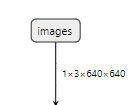
\includegraphics{figures/inputs.png}
\caption{Title of picture}
\end{figure}

\begin{figure}[H]
\centering
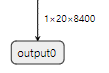
\includegraphics{figures/output.png}
\caption{Title of picture}
\end{figure}





#\begin{figure}[htbp]
#    \centering
#	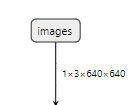
\includegraphics[width=0.5\textwidth]{figures/inputs.png}
#	\caption{"输入"}
#    \label{fig:input}
#\end{figure}
输出:
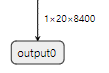
\includegraphics{figures/output.png}

在换脸的应用中,我会使用多个深度学习的网络,像是人脸关键点检测网络,换脸网络及人脸美化网络。他们有着类似的网络结果,所以,提取抽象类,封装为一个接口。
它通过定义纯虚函数强制派生类实现特定功能。

\begin{lstlisting}{c}
template <typename T>
class IEngine {
public:
    virtual ~IEngine() = default;
        const std::array<float, 3> &divVals = {1.f, 1.f, 1.f}, 
        bool normalize = true, int method = 0) = 0;
    virtual bool loadNetwork(
        std::string trtModelPath, 
        const std::array<float, 3> &subVals = {0.f, 0.f, 0.f},
        const std::array<float, 3> &divVals = {1.f, 1.f, 1.f}, 
        bool normalize = true) = 0;
    virtual bool runInference(
        const std::vector<std::vector<cv::cuda::GpuMat>> &inputs, 
        std::vector<std::vector<std::vector<T>>> &featureVectors) = 0;
    virtual const std::vector<nvinfer1::Dims3> &getInputDims() const = 0;
    virtual const std::vector<nvinfer1::Dims> &getOutputDims() const = 0;
};
\end{lstlisting}

定义Engine类实例化这个接口,实现接口定义的功能。
\begin{lstlisting}
	template <typename T>
class Engine : public IEngine<T> {
public:
    Engine(const Options &options);
    ~Engine();

    // Build the onnx model into a TensorRT engine file, cache the model to disk
    // (to avoid rebuilding in future), and then load the model into memory The
    // default implementation will normalize values between [0.f, 1.f] Setting the
    // normalize flag to false will leave values between [0.f, 255.f] (some
    // converted models may require this). If the model requires values to be
    // normalized between [-1.f, 1.f], use the following params:
    //    subVals = {0.5f, 0.5f, 0.5f};
    //    divVals = {0.5f, 0.5f, 0.5f};
    //    normalize = true;
    bool buildLoadNetwork(std::string onnxModelPath, const std::array<float, 3> &subVals = {0.f, 0.f, 0.f},
                          const std::array<float, 3> &divVals = {1.f, 1.f, 1.f}, bool normalize = true,int method = 0) override;

    // Load a TensorRT engine file from disk into memory
    // The default implementation will normalize values between [0.f, 1.f]
    // Setting the normalize flag to false will leave values between [0.f, 255.f]
    // (some converted models may require this). If the model requires values to
    // be normalized between [-1.f, 1.f], use the following params:
    //    subVals = {0.5f, 0.5f, 0.5f};
    //    divVals = {0.5f, 0.5f, 0.5f};
    //    normalize = true;
    bool loadNetwork(std::string trtModelPath, const std::array<float, 3> &subVals = {0.f, 0.f, 0.f},
                     const std::array<float, 3> &divVals = {1.f, 1.f, 1.f}, bool normalize = true) override;

    // Run inference.
    // Input format [input][batch][cv::cuda::GpuMat]
    // Output format [batch][output][feature_vector]
    bool runInference(const std::vector<std::vector<cv::cuda::GpuMat>> &inputs, std::vector<std::vector<std::vector<T>>> &featureVectors) override;

    // Utility method for resizing an image while maintaining the aspect ratio by
    // adding padding to smaller dimension after scaling While letterbox padding
    // normally adds padding to top & bottom, or left & right sides, this
    // implementation only adds padding to the right or bottom side This is done
    // so that it's easier to convert detected coordinates (ex. YOLO model) back
    // to the original reference frame.
    static cv::cuda::GpuMat resizeKeepAspectRatioPadRightBottom(const cv::cuda::GpuMat &input, size_t height, size_t width,
                                                                const cv::Scalar &bgcolor = cv::Scalar(0, 0, 0));

    [[nodiscard]] const std::vector<nvinfer1::Dims3> &getInputDims() const override { return m_inputDims; };
    [[nodiscard]] const std::vector<nvinfer1::Dims> &getOutputDims() const override { return m_outputDims; };

    // Utility method for transforming triple nested output array into 2D array
    // Should be used when the output batch size is 1, but there are multiple
    // output feature vectors
    static void transformOutput(std::vector<std::vector<std::vector<T>>> &input, std::vector<std::vector<T>> &output);

    // Utility method for transforming triple nested output array into single
    // array Should be used when the output batch size is 1, and there is only a
    // single output feature vector
    static void transformOutput(std::vector<std::vector<std::vector<T>>> &input, std::vector<T> &output);
    // Convert NHWC to NCHW and apply scaling and mean subtraction
    static cv::cuda::GpuMat blobFromGpuMats(const std::vector<cv::cuda::GpuMat> &batchInput, const std::array<float, 3> &subVals,
                                            const std::array<float, 3> &divVals, bool normalize, bool swapRB = false);

//private:
    // Build the network
    bool build(std::string onnxModelPath, const std::array<float, 3> &subVals, const std::array<float, 3> &divVals, bool normalize);
    bool build1(std::string onnxModelPath, const std::array<float, 3> &subVals, const std::array<float, 3> &divVals, bool normalize);

    bool constructNetwork(std::string onnxModelPath, std::unique_ptr<nvinfer1::IBuilder>& builder,
        std::unique_ptr<nvinfer1::INetworkDefinition>& network, std::unique_ptr<nvinfer1::IBuilderConfig>& config,
        std::unique_ptr<nvonnxparser::IParser>& parser);


    // Converts the engine options into a string
    std::string serializeEngineOptions(const Options &options, const std::string &onnxModelPath);

    void getDeviceNames(std::vector<std::string> &deviceNames);

    void clearGpuBuffers();

    // Normalization, scaling, and mean subtraction of inputs
    std::array<float, 3> m_subVals{};
    std::array<float, 3> m_divVals{};
    bool m_normalize;

    // Holds pointers to the input and output GPU buffers
    std::vector<void *> m_buffers;
    std::vector<uint32_t> m_outputLengths{};
    std::vector<nvinfer1::Dims3> m_inputDims;
    std::vector<nvinfer1::Dims> m_outputDims;
    std::vector<std::string> m_IOTensorNames;
    int32_t m_inputBatchSize;

    // Must keep IRuntime around for inference, see:
    // https://forums.developer.nvidia.com/t/is-it-safe-to-deallocate-nvinfer1-iruntime-after-creating-an-nvinfer1-icudaengine-but-before-running-inference-with-said-icudaengine/255381/2?u=cyruspk4w6
    //std::unique_ptr<nvinfer1::IRuntime> m_runtime = nullptr;
    std::shared_ptr<nvinfer1::IRuntime> m_runtime = nullptr;

    std::unique_ptr<Int8EntropyCalibrator2> m_calibrator = nullptr;
    //std::unique_ptr<nvinfer1::ICudaEngine> m_engine = nullptr;
    std::shared_ptr<nvinfer1::ICudaEngine> m_engine = nullptr;
    std::unique_ptr<nvinfer1::IExecutionContext> m_context = nullptr;
    const Options m_options;
    Logger m_logger;
};

template <typename T> Engine<T>::Engine(const Options &options) : m_options(options) {}

template <typename T> Engine<T>::~Engine() { clearGpuBuffers(); }

\end{lstlisting}




\LaTeX 的源文件本质上是文本文档,利用Windows自带文本编辑器、note++、word、vim等文本编辑器均可编写出tex文档,至于texwork、texstudio、winedt等则为转述的tex编辑器,提供了语法高亮、匹配查找、自动补全命令等等用途。

除此之外\LaTeX 还可以排版数学公式、图片、表格等等,内容将在后续章节件数。
\section{\LaTeX 基本的命令与代码结构}
\LaTeX 命令均由反斜线$\backslash$开头,并为下列两种形式填空后续:
\begin{itemize}
\item 由反斜线$\backslash$与一连串字母组成,如\verb|\LaTeX|。注意在命令后需加空格或其他非字母作分隔符;
\item 由反斜线$\backslash$由后面的非字母符号组成,不需要分隔符,如\verb|\%|(百分号在\LaTeX 中为注释),为转义意。
\end{itemize}

注意\LaTeX 命令对\textbf{大小写是十分敏感的},比如输入\verb|\LaTeX|可以得到错落有致的\LaTeX 而输入\verb|\LaTex|或者\verb|\latex|则会报错,不会得到任何内容。

在\LaTeX 中的参数大多在$\{\cdots\}$或是在$[\cdots]$内,如之前所述\verb|\documentclass|\texttt{[CJK, GBK, UTF-8, oneside, a4paper, 12pt]{ctexart}}。
一些命令会在后面附带*号,带*号与不带*号结果不同。

为使一些状态、效果在局部生效,\LaTeX 引入了\textbf{环境}的用法,需要局部生效的内容被输入在环境内,由\verb|\begin{environment name}{arguments}|开始,由\verb|\end{environment}|结束。其中$environment$为环境名称,\verb|\begin{environment}|与\verb|\end{environment}|内的环境名应该一致,$arguments$为可选参数,环境之间允许嵌套使用。
\section{\LaTeX 排版中文}
排版中文文章时,与word不同,无需关注缩进、标题等等,在\LaTeX 中可以方便快捷的设置。一级标题设置代码为\verb|\section{title}|大括号内为一级标题的名称,对应的可以书写二级、三级标题,\LaTeX 命令分别为\verb|\subsection{title}|与\verb|\subsubsection{title}|。书写时,\LaTeX 会自动忽略文字中间的空格,在换行时需要多空一行。另外的,\LaTeX 中的注释为“\%”号。下面给出一个简短的例子。
\begin{minted}{LaTeX}
\section{一级标题名称}
这里是第一章的内容
% 空一行代表分段,百分号在LaTeX中代表注释
这里是第一章的内容
\subsection{二级标题名称}
这里是1.1的内容
\end{minted}

用户可以将代码放置在本模板中进行尝试,需要注意的是,在body文件夹内新建文档并书写完后,需要在主文档中依照给定格式导入新书写的文档。

在\LaTeX 中书写中文,无需注意文章标题的编号,在\verb|\section{title}|类命令中,自带有计数器,可以为标题自动编号,这使得用户无需关注排版格式,更多的关注在文档内容上。
\section{常用环境}
\subsection{居中}
在\LaTeX 中有两种居中方式:
\begin{itemize}
\item \verb|\centering|,在环境内使用,该环境内所有内容居中
\item \verb|center| 环境,在环境内的所有内容居中
\end{itemize}
\begin{center}
当使用了\verb|center|环境时候,环境内的所有内容都会被居中显示,且不会首行缩进。如果有特殊需要还可以使用flushleft 和flushright 环境,用于居左或者居右。
\end{center}
\subsection{带有编号的显示方式-列表(悬挂缩进)}
在书写实验报告时,经常会遇到需要分条叙述的方式,在一般书写排版中需要整体悬挂缩进。

在\LaTeX 中常用的两种环境,分别是itemize(无序)环境与enumerate环境(有序)两种环境可以互相嵌套使用,使用方法如下:
\begin{minted}{LaTeX}
% itemize环境
\begin{itemize}
\item 第一条内容
\item 第二条内容
\end{itemize}
% enumerate环境
\begin{enumerate}[aa.]
\item 第一条内容
\item 第二条内容
\end{enumerate}
\end{minted}
itemize环境会给每一条内容前加$\bullet$,而enumerate环境可以自定义,如(1. 2. 3.或者是A. B. C.),对应的设置方法需要在环境后的参数中写\verb|1.|、\verb|A.|,需要注意的是在给enumerate环境添加参数时候需要导入enumerate包,否则只会有\verb|1. 2. 3.|的序号,并且无法设置样式。
\begin{itemize}
\item 第一条内容
\item 第二条内容
\end{itemize}
\begin{enumerate}[aa.]
\item 第一条内容第一条内容第一条内容第一条内容第一条内容第一条内容第一条内容第一条内容第一条内容第一条内容第一条内容第一条内容第一条内容第一条内容第一条内容第一条内容
\item 第二条内容
\end{enumerate}
\subsection{代码}
在实验报告中,多半部分需要加入对应的程序,编写代码的常用环境有verbatim、minted(需要python环境支持)、listings,下面分别叙述。

verbatim环境使用方法简单,但是不够美观,不能实现语法高亮。
\begin{verbatim}
#include<stdio.h>
int main(){
	printf("hello world");
	return 0;
}
\end{verbatim}

lstlisting环境需要listings包,可以自定义设置,本模板自带listings包并且给出了一种代码环境格式供用户参考。
\begin{lstlisting}{c}
#include<stdio.h>
int main(){
	printf("hello world");
	return 0;
}
\end{lstlisting}

minted环境需要minted包,并且电脑中安装有python环境。设置xelatex编译为\\\verb|xelatex.exe -synctex=1 -shell-escape -interaction=nonstopmode %.tex|,添加了\\\verb|-shell-escape|参数,可以胜任大部分计算机语言(Lingo除外),并且自动设置语法高亮。需要注意的是minted会将\verb|Tab|替换为下文中的\verb|^^I|,将所有的\verb|Tab|替换为空格即可,更多内容详见minted宏包文档,Win+R键后输入\verb|texdoc minted|即可查看minted宏包文档,在\LaTeX 中所有宏包的宏包文档均以上述方式打开。
\begin{minted}{C}
#include<stdio.h>
int main(){
	printf("hello world");
    return 0; /*将Tab替换为空格*/
}
\end{minted}

要排版简短的代码或关键字,可使用\verb|\verb| 命令:\verb|\verb<delim>\LaTeX<delim>|。
在该命令中所有的\verb|\|都不起作用。